\section{Configuração no ESP32}

Para a realização da prática, usamos um ESP32 de 30 pinos, uma protoboard de 400 pontos, um sensor ultrasônico HC-SR04, um LED RGB, dois resistores de 390 \textit{ohms}, sete cabos macho-fêmea e um cabo serial micro-USB.

Sem utilizar nenhum cabo, conectamos o HC-SR04 na protoboard. Deixamos ele bem perto da borda, pois é importante primeiro para questão de espaço na placa e para que nada fique entre ele e o objeto.


Aproveitamos para conecta-lo ao ESP32. O sensor possui quatro pinos. Um pino é o VCC que é para alimentação, então conectamos ele ao pino VIN do ESP32. O GND do sensor conectado ao GND do ESP. Os pinos de \textit{trigger} e de \textit{echo} podem ser conectados em qualquer pino de GPIO, e os pinos escolhidos foram o pino 5 para \textit{trigger} e o pino 18 para \textit{echo}. Usamos quatro cabos macho-fêmea.

\begin{figure}[H]
    \centering
    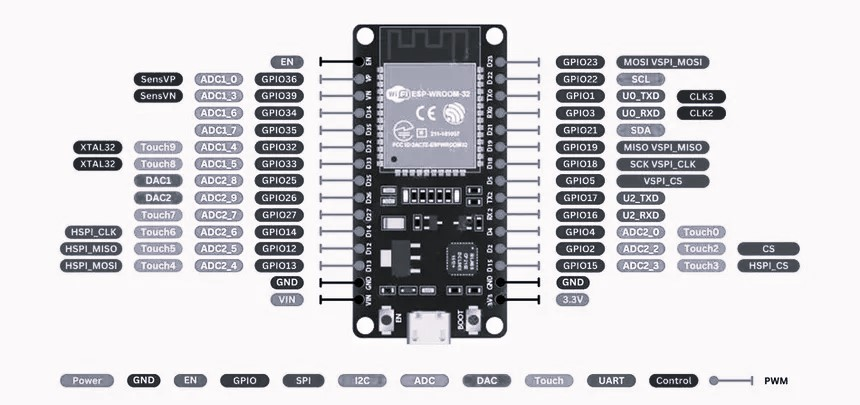
\includegraphics[width=0.5\linewidth]{img/esp32_pinout.png}
    \caption{Pinout do ESP32.}
    \label{fig:esp32-pinout}
\end{figure}

\begin{figure}[H]
    \centering
    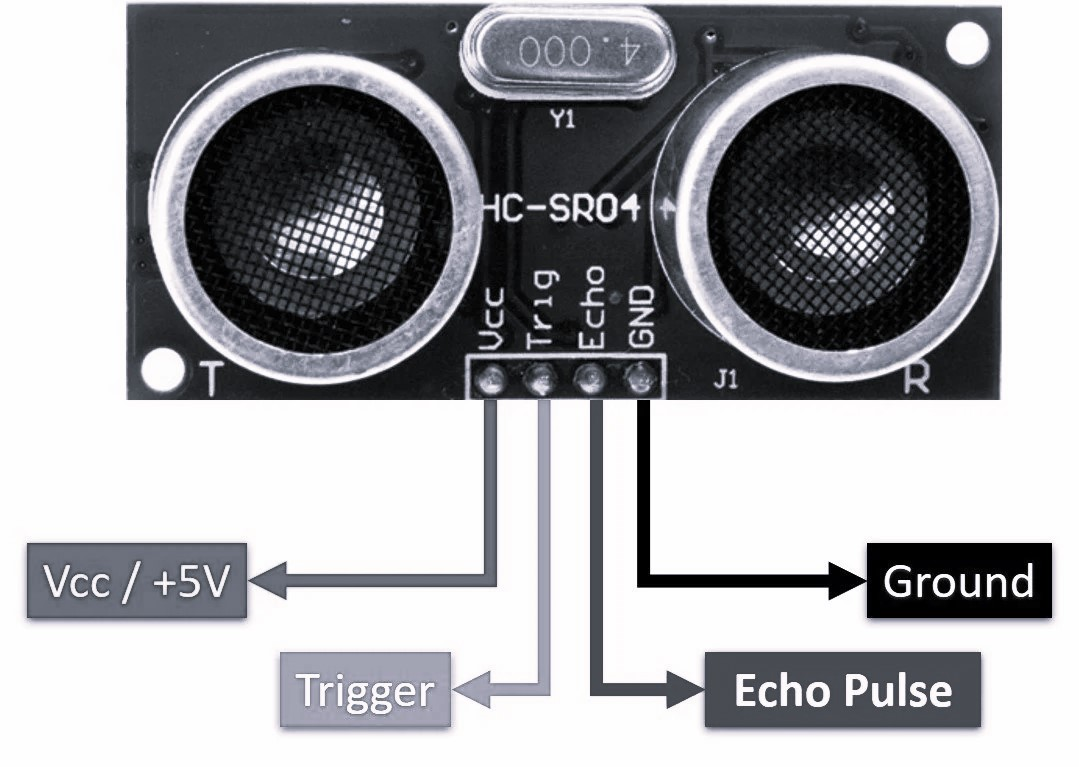
\includegraphics[width=0.5\linewidth]{img/HC-SR04-Ultrasonic-Sensor-Pinout.jpg}
    \caption{Pinout do sensor HC-SR04.}
    \label{fig:HC-SR04-pinout}
\end{figure}

O LED RGB é disposto num ponto próxima da beirada da protoboard para que seja possível inserir o pino do cátodo do LED na linha negativa, enquanto os outros pinos ficam em outros pontos da protoboard. Deixar o cátodo na linha negativa poderia facilitar caso precisassemos compartilhar o GND com o sensor, mas não foi necessário.

A configuração do LED RGB foi feita sem levar em conta o terminal do pino azul, visto que ele não será necessária para a realização da prática. Escolhemos os pinos 19 e 21 para conectá-los aos terminais vermelho e verde do LED. Isso antes de conectar os resistores nos terminais desses dois pinos. O cátodo do LED é ligado ao outro GND do ESP32. Assim, usamos os últimos dois cabos macho-fêmea.